% Use class option [extendedabs] to prepare the 1-page extended abstract.
\documentclass[extendedabs]{bmvc2k}
\usepackage[colorlinks = true,
            linkcolor = blue,
            urlcolor  = blue,
            citecolor = blue,
            anchorcolor = blue]{hyperref}
\usepackage{kotex}
% for the fancy \koTeX logo
\usepackage{kotex-logo}
\usepackage{mathtools}  % brings in amsmath, also some improvements
\usepackage{amssymb} % brings in amsfonts, incl \square
% Document starts here
\begin{document}


\title{semantic segmentation final-report}
\addauthor{
Taehun Kim$^{1}$
}{}{1}

\addinstitution{
$^1$ Department of Computer Science and Engineering, Pusan National University.  
}
 

\maketitle
\noindent

\begin{figure}[t]
	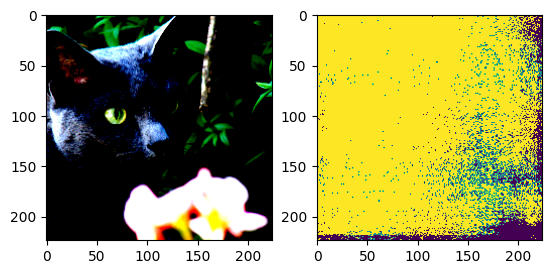
\includegraphics[width=\linewidth]{images/fig1.png}
	\caption{
		patch-wise semantic segmentation of a Egyptian cat image. normalized image(left) and pixel-to-pixel classification results(right). a yellow pixel indicate that the pixel is the Egyptian cat class, a purple pixel indicate that the pixel is not the Egyptian cat class.}
        \label{fig:patch-wise}
	\vspace{-2mm}
\end{figure}
\begin{figure}[t]
	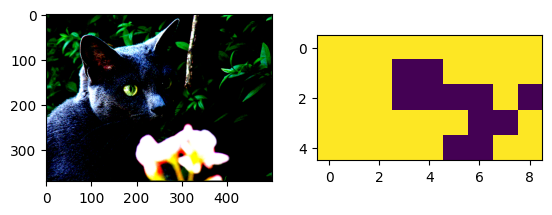
\includegraphics[width=\linewidth]{images/fig2.png}
	\caption{
		pixel-wise semantic segmentation of a Egyptian cat image. classification results are sparse because the final output features of VGG-16\cite{vggnet} is 32 times smaller than the input image. normalized image(left) and pixel-to-pixel classification results(right). a yellow pixel indicate that the pixel is the Egyptian cat class. a purple pixel indicate that the pixel is not the Egyptian cat class.}
        \label{fig:pixel-wise}
	\vspace{-2mm}
\end{figure}
\begin{figure}[t]
	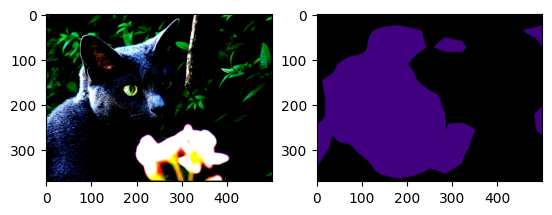
\includegraphics[width=\linewidth]{images/fig3.png}
	\caption{
		pixel-wise semantic segmentation (with bilinear interpolation) of a Egyptian cat image. normalized image(left) and pixel-to-pixel classification results(right). a purple pixel indicate that the pixel is the Egyptian cat class. a black pixel indicate that the pixel is not the Egyptian cat class. The last fully convolutional layers are random-initialized.}
        \label{fig:pixel-wise-bilinear}
	\vspace{-2mm}
\end{figure}

\section{Introduction}
Fully Convolutional Networks\cite{fcn} are semantic segmentation networks that classify all pixels in image by replacing fully connected layers to convolutional layers in VGG-16\cite{vggnet} and using skip connections.

We implement the FCN-8s introduced in the Fully Convolutional Network paper\cite{fcn} with VGG-16, train with PASCAL VOC 2012 dataset, analyze and discuss the result.

\section{patch-wise vs. pixel-wise} \label{previousmodel}
Before implementing FCN-8s, we did a simple experiment that compare patch-wise segmentation and pixel-wise segmentation.
\subsection{patch-wise segmentation}\label{patchwisesec}
We picked up a Egyptian cat image(2009\_005160.jpg in the PASCAL VOC 2012 dataset), resize it to 256, cut into 224 around the center, and normalize with Imagenet mean and standard.
Also, this image is padded 111 pixels on top and left sides, and padded 112 pixels on bottom and right sides.

After padding, a sliding window of size $224\times224$ is applied, and each window fed into a pre-trained VGG-16\cite{vggnet} model to predict the class of the central pixel of the sliding window. The results is shown on figure \ref{fig:patch-wise}. The result is inaccuracy. Also, this method is inefficient because all sliding windows are fed into a convolutional network individually.
\subsection{pixel-wise segmentation} \label{pixelwisesec}
We selected the Egyptian cat image and preprocessed it in the same way as described in the patch-wise segmentation section above. \ref{patchwisesec}

We replaced the fully connected layers in pretrained VGG-16\cite{vggnet} with convolutional layers. The architecture of the Fully-Convolutional-VGG16 is shown on Table \ref{tab:convvgg}. The added convolutional layers were initialized with the weights of the fully connected layers from the pretrained VGG-16\cite{vggnet} network.

Output of this network with Egyptian cat image as input is shown in Figure \ref{fig:pixel-wise}. The output of this network is much smaller than the original image resolution and many pixels are misclassified. this is because the output features of VGG-16 are 32 times smaller than the input image.
\begin{table}[]
\centering
\begin{tabular}{|c|}
\hline
$h \times w$ image padded by 111-112 pixel on all four sides \\ \hline
pretrained-VGG-16 features network                                        \\ \hline
conv7-4096 no-pad                                                         \\ \hline
ReLU                                                                      \\ \hline
Dropout                                                                   \\ \hline
conv1-4096 no-pad                                                         \\ \hline
ReLU                                                                      \\ \hline
Dropout                                                                   \\ \hline
conv1-1000 no-pad                                                         \\ \hline
\end{tabular}
\caption{The architecture of the convolutional VGG Network for pixel-wise classification. convx-y indicates convolution layer that has $x\times x$ filter and the number of the output channel is $y$}
\label{tab:convvgg}
\end{table}

\subsection{adding upsampling layer and retrain with PASCAL VOC} \label{addupsample}
The network is similar to the previously defined architecture in \ref{pixelwisesec}. the number of the output channel of last fully convolutional layer is 21 because PASCAL VOC 2012 dataset has 20 classes and we should classify the background(+1). We also apply bilinear interpolation to the output of the last layer so that the output resolution matches the input resolution. The network architecture is shown in \ref{tab:bilinearvgg}. The output shape is changed from $(h/32 \times w/32 \times 21)$ to $(h\times w\times 21)$ by bilinear interpolation. The first two fully convolutional layers are initialized with weight of the first two fully connected layers of VGG-16\cite{vggnet}. The last fully convolutional layers are intialized randomly. The result of this network is shown on figure \ref{fig:pixel-wise-bilinear}. The network is more accurate than previous network, but 32 times bilinear interpolation limits the scale of detail in the upsampled output.

\section{FCN-8s}
To improve the scale of details in upsampled output, We need prediction from shallower layers in VGG-16. Because shallower layers produce finer outputs and better detect the location of objects. On the other hand, deeper layers produce coarse outputs and better detect the type of objects because the information is compressed as the image passes through the convolution layers. So we need to combine prediction of shallower layers and deeper layers. One of the combined prediction architecture is FCN-8s.

The architecture of FCN-8s is shown in figure \ref{fig:fcn-8sarch}. We use pretrained VGG-16, and the last fully convolutional layers are replaced to fully convolutional layers and initialized same as \ref{addupsample}. We first add a $1\times1$ convolutional layers with 21 channels output on top of output after fourth maxpooling. this convolutional layer predict class probability of each output after forth maxpooling. Second, output of last layers(prediction from last layer) is 2x upsampled.

Third, prediction from fourth maxpooling and last layer are combined with weight of the fourth maxpooling is 0.01. Fourth, this combined prediction is 2x upsampled. Fifth, we add a $1\times1$ convolutional layers with 21 channels output on top of output after third maxpooling. The prediction from third maxpooling and the combined prediction are combined with weight of the prediction from third maxpooling is 0.0001.

We use bilinear interpolation(not transpose convolution) as upsampling method. Additionally, if the shapes of the two predictions are different, we crop the larger prediction to match the size of the smaller prediction.

\subsection{Dataset}
To train the FCN-8s, we use the PASCAL VOC 2012 dataset. This dataset contains 10,582 training images and 1,449 testing images. It includes 20 classes, such as aeroplane, car, cat, cow, and person. The dataset provides both images and ground truth data, where the ground truth data specifies the class of each pixel(with class of background is 0). additionally, all image are resized to $321\times321$
\subsubsection{Data pre-processing}
For data augmentation, We flip the image with 50\% probability, and resize the image randomly to a scale between 0.5x and 1.3x. the resizing method for image is INTER-LINEAR, and the method for ground-truth is INTER-NEAREST.
\subsection{Training}
The first two fully convolutional layers are initialized with models provided in advance. The learning rate is $10^{-4}$, and we use adam optimizer. The loss function is cross entropy, and the model is trained for 10 epochs.

We trained the FCN-8s model using three different approaches: in the VGG16 features network, all layers are not fixed, only the last 10 layers are trainable, and all layers are fixed.

\subsection{Testing and Result}
We test the model with PASCAL VOC 2012 test images. The mean IoU of each model is shown in Table \ref{tab:fcn8sresult}. The mean IoU is highest at 0.4952 when the entire feature network of VGG-16 in FCN-8s is fixed. The inference result of test image using this model is shown in Figure \ref{fig:inferresult}, Figure \ref{fig:inferresult2}, Figure \ref{fig:inferresultinaccuracy}. The result is more accurate than previous model in section \ref{previousmodel}. However, From Figure \ref{fig:inferresultinaccuracy}, We can identify the limitations of FCN. As described in Learning Deconvolution Network paper\cite{learningdeconv}, FCN has weaknesses in detecting small object and objects that belong to the another large object. this is because the network can handle a single scale semantic due to the fixed receptive field.

\section{conclusion}
We implement a patch-wise, pixel-wise, FCN-32s, and FCN-8s. We also train, test the FCN-8s model with PASCAL VOC 2012 dataset and analyze the result. The FCN-8s with a fixed VGG-16 feature network has the highest performance(0.4952 mean IoU). However this model has limitation in detecting small object and objects belong to the large object, This model can detect type and location of the object more accurate than patch-wise, pixel-wise and FCN-32s. This model also can detect contour of the object quite accurate. As a result, We confirm that Fully Convolutional Network can semantic segmentation beyond image classification.
\begin{figure}[t]
	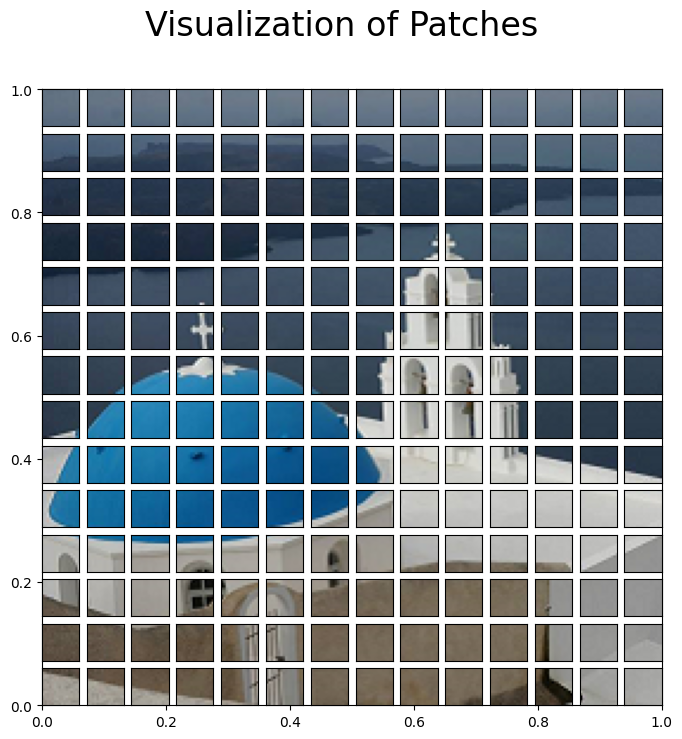
\includegraphics[width=\linewidth]{images/fig4.png}
	\caption{
		architecture of FCN-8s. First, the fully connected layers in VGG-16 is replaced to fully convolutional layers. Second, output of last layer is 2x upsampled and added to prediction after 4 maxpooling. Third, the combined prediction is 2x upsampled and added to prediction after 3 maxpooling. Finally the combined prediction is 8x upsampled. }
        \label{fig:fcn-8sarch}
	\vspace{-2mm}
\end{figure}

\begin{table}[]
\centering
\begin{tabular}{|c|}
\hline
input:  $h \times w$ image padded by 100 pixel on all four sides \\ \hline
pretrained-VGG-16 features network                    \\ \hline
conv7-4096 no-pad                                     \\ \hline
ReLU                                                  \\ \hline
Dropout                                               \\ \hline
conv1-4096 no-pad                                     \\ \hline
ReLU                                                  \\ \hline
Dropout                                               \\ \hline
conv1-21 no-pad                                       \\ \hline
bilinear interpolation                                \\ \hline
\end{tabular}
\caption{The architecture of the convolutional VGG Network with upsampling for pixel-wise classification of PASCAL VOC 2012 dataset.}
\label{tab:bilinearvgg}
\end{table}

\begin{table}[t]
\centering
\begin{tabular}{|l|l|}
\hline
VGG-16 configuration                     & mean IoU of test images \\ \hline
all features layers are not fixed        & 0.2073                 \\ \hline
last 10 layers of features are trainable & 0.4048                  \\ \hline
All layers of feature network is fixed      & 0.4952                  \\ \hline
\end{tabular}
\caption{The test results of the FCN-8s models using three different approaches in the VGG-16 feature network.}
\label{tab:fcn8sresult}
\end{table}

\begin{figure}[t]
\centering
	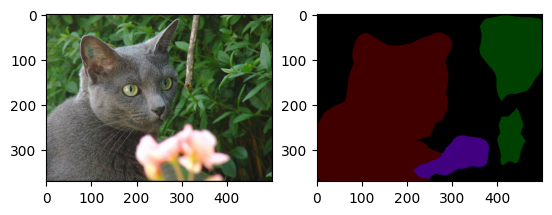
\includegraphics[width=0.7\linewidth]{images/result/result1.png}
    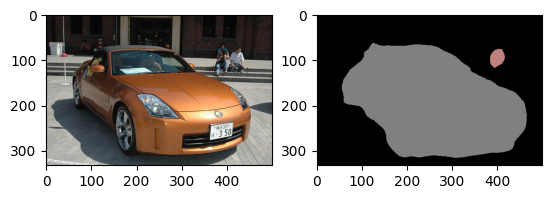
\includegraphics[width=0.7\linewidth]{images/result/result2.png}
    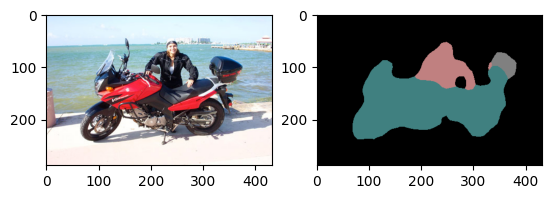
\includegraphics[width=0.7\linewidth]{images/result/result3.png}
    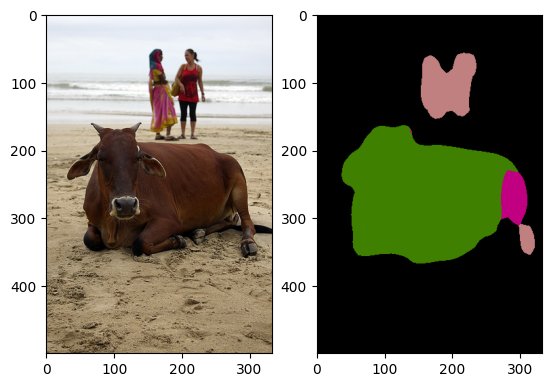
\includegraphics[width=0.7\linewidth]{images/result/result4.png}
    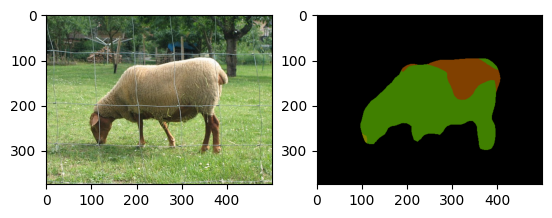
\includegraphics[width=0.7\linewidth]{images/result/result5.png}
    
	\caption{
		The results of semantic segmentation on PASCAL VOC 2012 images using the trained FCN-8s model. }
        \label{fig:inferresult}
	\vspace{-2mm}
\end{figure}



\begin{figure}[t]
\centering
	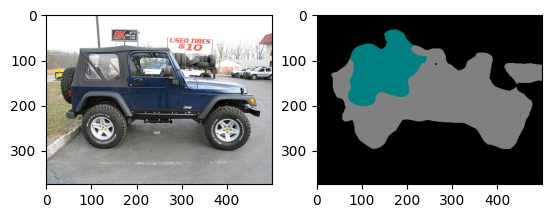
\includegraphics[width=0.7\linewidth]{images/result/result6.png}
    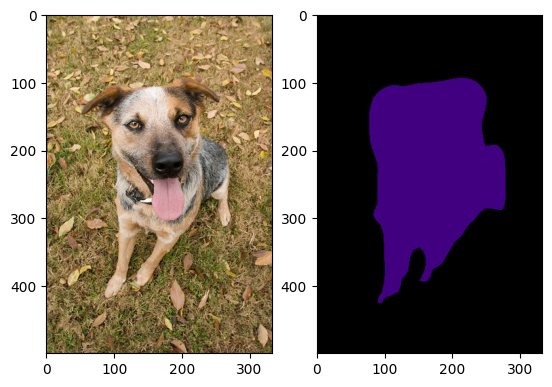
\includegraphics[width=0.7\linewidth]{images/result/result7.png}
    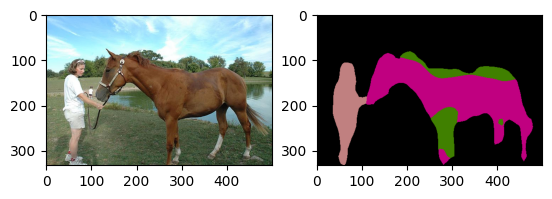
\includegraphics[width=0.7\linewidth]{images/result/result8.png}
    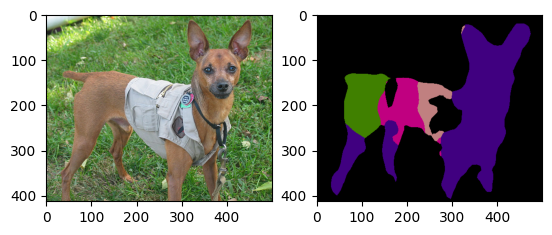
\includegraphics[width=0.7\linewidth]{images/result/result9.png}
    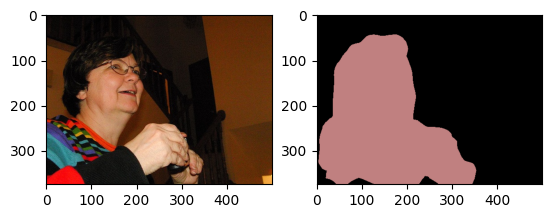
\includegraphics[width=0.7\linewidth]{images/result/result10.png}
    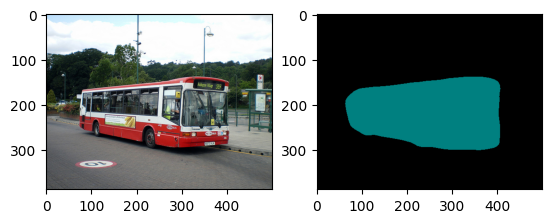
\includegraphics[width=0.7\linewidth]{images/result/result11.png}
    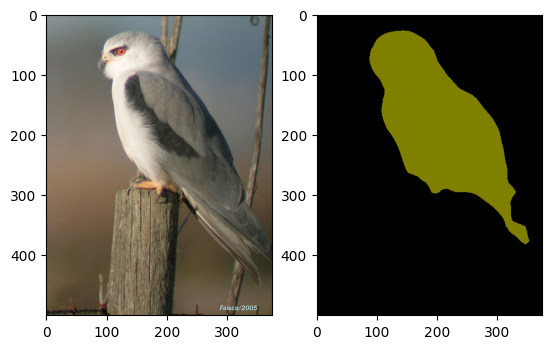
\includegraphics[width=0.7\linewidth]{images/result/result12.png}
    
	\caption{
		The results of semantic segmentation on PASCAL VOC 2012 images using the trained FCN-8s model. }
        \label{fig:inferresult2}
	\vspace{-2mm}
\end{figure}

\begin{figure}[t]
	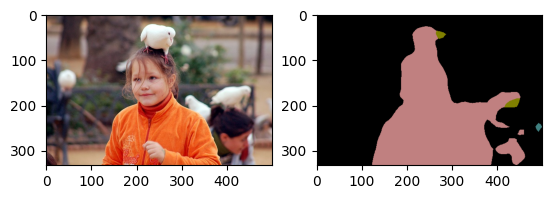
\includegraphics[width=\linewidth]{images/result/result13.png}
    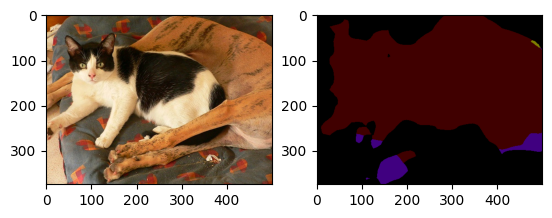
\includegraphics[width=\linewidth]{images/result/result14.png}
    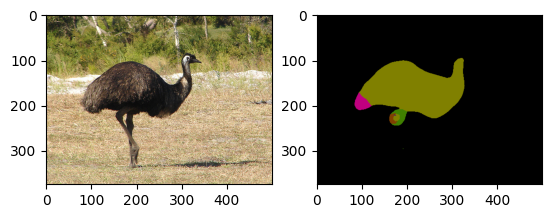
\includegraphics[width=\linewidth]{images/result/result15.png}

	\caption{
		The results of semantic segmentation on PASCAL VOC 2012 images using the trained FCN-8s model. This model has weaknesses in detecting small objects and objects that belong to the another large object.  }
        \label{fig:inferresultinaccuracy}
	\vspace{-2mm}
\end{figure}

\newpage
\bibliography{egbib}

\end{document}
